\documentclass[12pt,a3paper, foldmark,notumble]{leaflet}
\usepackage[none]{hyphenat}
\usepackage[utf8]{inputenc}
\usepackage[T1]{fontenc}
\usepackage[francais]{babel}
\usepackage{libertine}
\renewcommand{\familydefault}{\sfdefault}
\usepackage{microtype}
\usepackage{menukeys}
\usepackage{flowfram,graphicx}
\usepackage{fontawesome}
\usepackage{courier}
\usepackage{titlesec}
\usepackage{color}
\usepackage{verbatim}
\usepackage{enumitem}
\usepackage{wallpaper}
\usepackage[most,listings]{tcolorbox}
\usepackage{qrcode}
\usepackage{wrapfig,rotating}
\usepackage{adjustbox}
\usepackage{csquotes}
\usepackage{framed}
\usepackage[colorlinks=false, urlcolor=black, hidelinks]{hyperref}
\usepackage{qrcode}

\setitemize{label=--}
\setenumerate[1]{label=\textcircled{\scriptsize\arabic*},
  font=\sffamily}
\pagenumbering{gobble}
\CutLine*{3}
\CutLine*{4}
\CutLine*{6}
\CutLine*{1}



% Colors
\definecolor{red}{cmyk}{0, 1, 1, 0}

% Text Heading Color
% orange {0,0.69,1,0}
% {0.08, 0.47, 0, 0.33}
% {1, 0.56, 0, 0}
% {0.94, 1, 0, 0} 
% {0.44, 1, 0, 0}
% {0, 1, 0.06, 0} Pink
% {1, 0.58, 0, 0.33} Cobalt Blue
% {1, 0.58, 0, 0.03}
% Dark Magenta {0, 1, 0, 0.45}
% Blue {0.83, 0.74, 0, 0.11}
% 	{0.25, 0.50, 0, 0.20}

% New colors
%\definecolor{orange}{cmyk}{0, 1, 0.06, 0}
%\definecolor{orange}{cmyk}{0.61, 0.20, 0, 0.44}
%\definecolor{orange}{cmyk}{0.67, 0.30, 0, 0.56}

%\definecolor{orange}{cmyk}{0.86, 0.64, 0, 0}
\definecolor{orange}{cmyk}{	0, 1, 1, 0}

% Outer Border Color
% olive {0.31,0,1,0.71}
% green {0.40, 0, 0.47, 0.33}
% {0, 0.92, 1, 0.03}
% {0, 0.92, 1, 0.42}
% olive 0.40, 0, 0.47, 0.33

% New colors
%\definecolor{olive}{cmyk}{0.20, 0.83, 0, 0.24}
%\definecolor{olive}{cmyk}{0.61, 0.20, 0, 0.44}

%\definecolor{blue}{cmyk}{1,1,0,0.8}
%\definecolor{green}{cmyk}{0.389,0,0.884,0.627}


%%%%%%%%%%%%%%%%%%%%%%%%%%%%%%%%%%%
% Border + Text Color combinations:
%%%%%%%%%%%%%%%%%%%%%%%%%%%%%%%%%%%

%\definecolor{orange}{cmyk}{0.61, 0.20, 0, 0.44}
%\definecolor{olive}{cmyk}{0.61, 0.20, 0, 0.44}

%\definecolor{orange}{cmyk}{0.67, 0.30, 0, 0.56}
%\definecolor{olive}{cmyk}{0.61, 0.20, 0, 0.44}

%\definecolor{orange}{cmyk}{0, 0.72, 0.71, 0.64}
%\definecolor{olive}{cmyk}{0, 0.72, 0.71, 0.64}

%\definecolor{orange}{cmyk}{0, 0.76, 0.39, 0.45}

%\definecolor{olive}{cmyk}{0, 0.76, 0.39, 0.45}
%\definecolor{olive}{cmyk}{0, 1, 1, 0}

%\definecolor{orange}{cmyk}{0.19, 0.10, 0, 0.51}
%\definecolor{olive}{cmyk}{0.19, 0.10, 0, 0.51}

\definecolor{orange}{cmyk}{0, 0.66, 0.42, 0.35}
\definecolor{olive}{cmyk}{0, 0.66, 0.42, 0.35}

%\definecolor{orange}{cmyk}{0, 0.07, 0.20, 0.62}
%\definecolor{olive}{cmyk}{0, 0.07, 0.20, 0.62}

%\definecolor{orange}{cmyk}{0.48, 0, 0.37, 0.53}
%\definecolor{olive}{cmyk}{0, 0.38, 0.88, 0.24}

%\definecolor{orange}{cmyk}{0.56, 0.38, 0, 0.10}
%\definecolor{olive}{cmyk}{0.56, 0.38, 0, 0.10}

%\definecolor{orange}{cmyk}{0.65, 0.45, 0, 0.46}
%\definecolor{olive}{cmyk}{0.65, 0.45, 0, 0.46}

\titlespacing\section{0pt}{12pt plus 6pt minus 2pt}{0pt plus 2pt minus 2pt}
\titleformat{\section}
{\color{orange}\normalfont\normalsize\bfseries}
{\color{orange}\thesection}{1em}{}


\newcommand*\openquote{\makebox(25,-22){\scalebox{5}{}}}
\newcommand*\closequote{\makebox(25,-22){\scalebox{5}{}}}

\colorlet{shadecolor}{green}

\makeatletter
\newif\if@right
\def\shadequote{\@righttrue\shadequote@i}
\def\shadequote@i{\begin{snugshade}\begin{quote}\openquote}
		\def\endshadequote{%
			\if@right\hfill\fi\closequote\end{quote}\end{snugshade}}
\@namedef{shadequote*}{\@rightfalse\shadequote@i}
\@namedef{endshadequote*}{\endshadequote}
\makeatother


\TileSquareWallPaper{1}{7}

\setmargins{10mm}{10mm}{5mm}{5mm}
\vtwotonetop{0.5cm}{0.6\paperwidth}{olive}{topleft}{0.4\paperwidth}{olive}{topright}
\vtwotonebottom{0.5cm}{0.6\paperwidth}{olive}{bottomleft}{0.4\paperwidth}{olive}{bottomright}

%%%%%%%%%%%%%%%%%%%%%%%%%%%%%%%%%%%%%%%%%%%%%%%%%%%%%%%%%%%%%%%%%%%%%%%%%%%%%%%%%%%%%%%%%%%%%%%%%%%%%%%%%%%%%%%%%%%%%%%%%%%%%%%%%%%%%%%%%%%%%%%%%%%%%%%%%%%%%%%%%%%%%%%%%
%	PAGE-1
%%%%%%%%%%%%%%%%%%%%%%%%%%%%%%%%%%%%%%%%%%%%%%%%%%%%%%%%%%%%%%%%%%%%%%%%%%%%%%%%%%%%%%%%%%%%%%%%%%%%%%%%%%%%%%%%%%%%%%%%%%%%%%%%%%%%%%%%%%%%%%%%%%%%%%%%%%%%%%%%%%%%%%%%%

%\ThisTileWallPaper{1\paperwidth}{1\paperheight}{1}
\begin{document}
\begin{center}
	\textbf{\color{orange} {\LARGE $\text{2}^{\text{nd}}$ National Conference on Communication Systems}}\\
	\textbf{\color{orange} {\LARGE (Virtual Mode)}}\\
	\textbf{\color{orange} {\LARGE November 21, 2020}}\vspace{0.25cm}\\
	
\includegraphics[scale=0.30,trim={0cm, 4cm, 0cm, 3cm},clip]{Logo2.pdf} \vspace{-0.20cm}\\
	\textbf{\color{orange} {\Large \textit{Signal Processing and Machine Learning Techniques for Communication}}}\\ \vspace{0.25cm}
	\textbf{{\color{black}{\Large in association with}}}\\ \vspace{0.25cm}
	
\includegraphics[scale=0.375]{two_logos.eps}\\ \vspace{0.25cm}
	\textbf{{\color{orange}{\Large Indian Society for Technical Education, \\New Delhi}}} \\
	\textbf{\color{black}{\large Under the Societies Registration Act XXI of 1860}}\vspace{0.25cm}\\
	\textbf{{\color{orange}{\Large\&}}} \vspace{0.25cm}\\
	\textbf{{\color{orange}{\Large The Institution of Engineers (India)}}}\\ 
	\textbf{\color{black}{\large Established 1920, Incorporated by Royal Charter 1935}}\\
	\textbf{\color{black}{\large Puducherry State Centre, Puducherry}} \\\vspace{0.5cm}
	\textbf{{\color{black}{\Large Organized by} }}\\ \vspace{0.25cm}
	\textbf{{\color{orange}{\Large Department of Electronics and Communication Engineering}}}
\end{center}



\begin{center}
	{
\includegraphics[height=3.5cm,keepaspectratio]{NITPYlogo}}
\end{center}
\vspace{-0.70cm}
\begin{center}
	\textbf{{\color{orange}{\Large National Institute of Technology Puducherry\\ Thiruvettakudy, Karaikal, 609 609, India}}}\\ 
	\textbf{{\color{orange}{\large  An Institution of National Importance\\ under Ministry of Education, Government of India}}}\\
	\textbf{{\color{orange}{\large  Telefax: +91 4368 265230, Website: www.nitpy.ac.in}}}	
\end{center}

%%%%%%%%%%%%%%%%%%%%%%%%%%%%%%%%%%%%%%%%%%%%%%%%%%%%%%%%%%%%%%%%%%%%%%%%%%%%%%%%%%%%%%%%%%%%%%%%%%%%%%%%%%%%%%%%%%%%%%%%%%%%%%%%%%%%%%%%%%%%%%%%%%%%%%%%%%%%%%%%%%%%%%%%%
%	PAGE-2
%%%%%%%%%%%%%%%%%%%%%%%%%%%%%%%%%%%%%%%%%%%%%%%%%%%%%%%%%%%%%%%%%%%%%%%%%%%%%%%%%%%%%%%%%%%%%%%%%%%%%%%%%%%%%%%%%%%%%%%%%%%%%%%%%%%%%%%%%%%%%%%%%%%%%%%%%%%%%%%%%%%%%%%%%

\clearpage
\section{\faUniversity~ \textbf{About NIT Puducherry, Karaikal}}
\begin{center}
	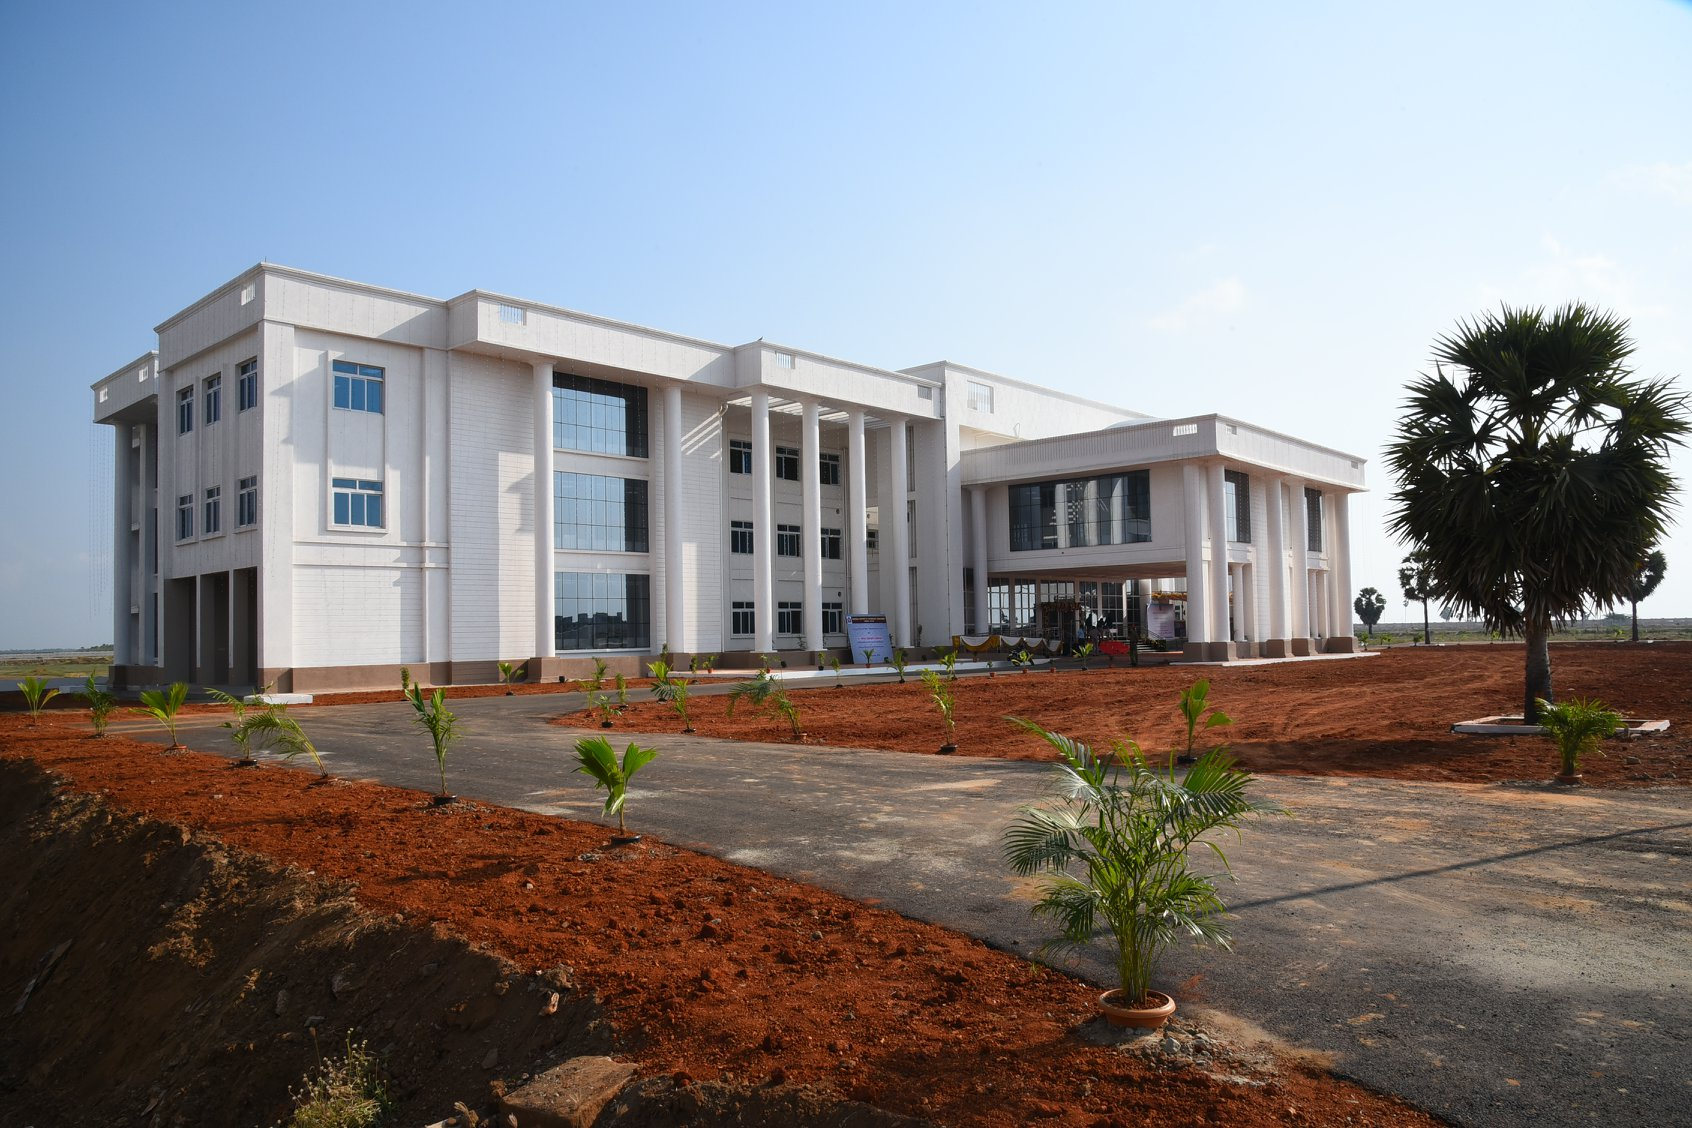
\includegraphics[scale=0.215,trim={0cm, 14cm, 0cm, 6cm},clip]{admin.jpg}	
\end{center}
National Institute of Technology Puducherry, Karaikal (NITPY), is an autonomous public engineering institute nestled in the scenes of Karaikal, a coastal enclave in the basin of river Kaveri in the Union Territory of Puducherry. It is one among the 31 National Institutes of Technology of India, and is declared as an institute of national importance by the Government of India, under NIT Act, 2007. The institute was established in 2010, starting its intake in the academic year 2010-11. NIT Puducherry is having a campus spread around 258 acres in the village Poovam and Thiruvettakudi of Karaikal. The institution is at a constant attempt of making endeavours to scale new heights by developing a synergy between studies, research, consulting/training activities, and placements. The institute is ranked at $130$ under the category of \enquote*{India Rankings 2020 - Engineering} of the 2020 NIRF rankings, released by the erstwhile Ministry of Human Resource Development, Government of India. 


\section{\faUniversity~ \textbf{About the Department of ECE}}
\begin{center}
	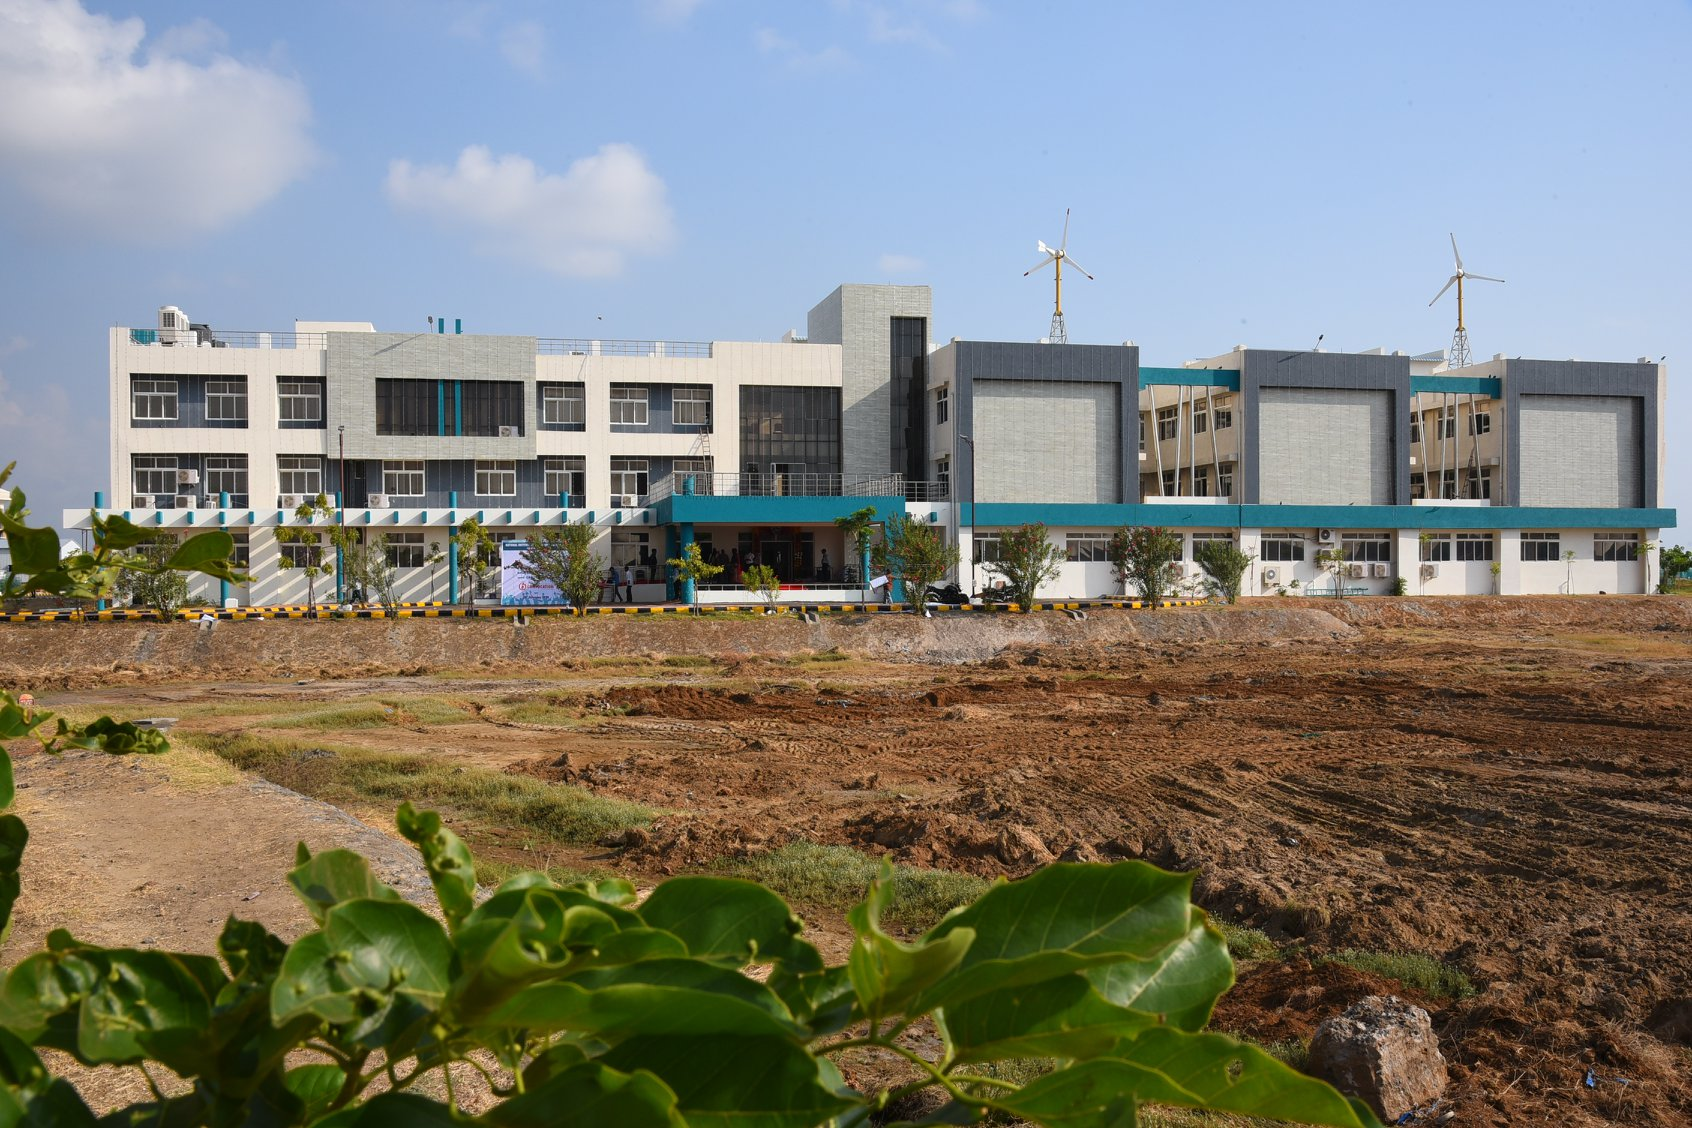
\includegraphics[scale=0.215,trim={0cm, 16cm, 0cm, 6cm},clip]{scb.jpg}	
\end{center}
The Department of Electronics and Communication Engineering offers UG, PG and Ph.D. courses, with a vision to promote research \& development in the frontier areas of electronics \& communication engineering and technology. The mission of the department is to enable the students to innovate and excel as eminent academicians, technocrats and entrepreneurs. The department has commissioned a new M.Tech course in VLSI Design from the academic year 2020-21. The department has numerous research scholars who are working in the institute/sponsored/funded projects of diverse research fields.

\section{\faBank~ About NCOCS-2020}
The idea behind NCOCS is to promote research \& development in the field of communication engineering and technology in India. The aim of this conference is to bring academicians, researchers, startups, and industrial practitioners together to exchange their ideas in the area of communications. The $1^{st}$ edition of NCOCS began in September 2019. It was a grand success with positive feedback from the participants. With an overwhelming response, the organizing team is going to make a second milestone of the NCOCS, in November 2020. With great support, the team is going to connect globally for exchanging the ideas in the field of machine learning and artificial intelligence for communication systems. 
Keeping in view of the unprecedented pandemic situation created due to COVID-19, the competent authority had decided to conduct the $2^{nd}$ edition of NCOCS in virtual mode. 
%Therefore, participants are required to equip with Laptop/PC/Mobile having internet connectivity. The registered participants will receive further details regarding the online platform and login credentials via e-mail.     

%%%%%%%%%%%%%%%%%%%%%%%%%%%%%%%%%%%%%%%%%%%%%%%%%%%%%%%%%%%%%%%%%%%%%%%%%%%%%%%%%%%%%%%%%%%%%%%%%%%%%%%%%%%%%%%%%%%%%%%%%%%%%%%%%%%%%%%%%%%%%%%%%%%%%%%%%%%%%%%%%%%%%%%%%
%	PAGE-3
%%%%%%%%%%%%%%%%%%%%%%%%%%%%%%%%%%%%%%%%%%%%%%%%%%%%%%%%%%%%%%%%%%%%%%%%%%%%%%%%%%%%%%%%%%%%%%%%%%%%%%%%%%%%%%%%%%%%%%%%%%%%%%%%%%%%%%%%%%%%%%%%%%%%%%%%%%%%%%%%%%%%%%%%%

\section{\faHandORight~   \textbf{Objectives:}}
To bring together researchers, young faculties and practitioners working in multi-disciplinary fields to discuss and deliberate on challenges, opportunities and strategies involved for communication systems. The conference will provide a global forum to academic researchers and practitioners to discuss critical issues concerning latest technologies.

\section{\faNewspaperO~  Call  for Papers}
Prospective authors are invited to submit manuscripts reporting original, unpublished research and recent developments in the topics related to the conference. Submissions must include title, abstract, author affiliation with the email address and keywords as per the recommended template. Regular Papers (6 pages in length) should present novel perspectives with in the general scope of the conference. Short papers (4 pages in length) are an opportunity to present preliminary or interim results. Submitted papers are limited to the maximum of 6 pages in length, and the typeset should be in standard IEEE conference format. Literature reviews/ survey papers will only be considered if they present a new perspective or benefit the field. To be published, such papers must go beyond view of the literature to define the field in a new way or highlight exciting new technologies or areas of research. The recommended paper templates for NCOCS-2020 can be downloaded using the links provided below.

\subsection{Templates:}
\faHandORight~\href{https://www.ieee.org/content/dam/ieee-org/ieee/web/org/conferences/Conference-LaTeX-template_7-9-18.zip}{ Click here for \LaTeX template} \hspace{0.75cm}
\faHandORight~\href{https://www.ieee.org/content/dam/ieee-org/ieee/web/org/conferences/conference-template-a4.docx}{Click here for MS Word template}

\section{\faCloudUpload~  Paper Submission}

\includegraphics[scale=0.30]{easychair}

Authors must submit their manuscripts through EasyChair.
\begin{itemize}
	\item[\faHandORight ] \href{https://easychair.org/conferences/?conf=ncocs2020}{Click here to submit your manuscript for NCOCS-2020}
\end{itemize}

\section{\faGroup~  \textbf{Who can participate}}
Professionals from various segments of the Industries, Consultants, University Faculties, Scientists from R\&D Institutions, Research Scholars, Students and Corporate Practitioners can attend and present their research articles.

\section{\faBullseye~ Topics of Interests}
Researchers working in the emerging fields of communication engineering and technology are encouraged to submit their original research findings. NCOCS-2020 welcomes original and unpublished research papers in the following topics but are not limited to,
\vspace{0.18cm}
\begin{tcolorbox}[colframe=olive,title= {}]
	\textbf{ 
		\begin{itemize}
			\item Wireless Sensor Networks;
			\item Wireless Communications;
			\item Physical Layer Modelling;
			\item MAC Layer Protocols;
			\item Channel Estimation;
			\item Machine Learning;
			\item Communication Systems for 5G and Beyond; 
			\item Underwater Sensor Networks;
			\item Internet of Things;
			\item Internet of Vehicles;
			\item Computer Communications;
			\item Antenna and Wave Propagation;
			\item RF \& Microwave Communications;
			\item Satellite and Optical Communications;
			\item Signal Processing;
			\item Image Processing;
			\item Audio and Video Signal Processing;
			\item Speech Processing;
			\item Embedded Systems;
			\item VLSI;
	\end{itemize}}
\end{tcolorbox}



%%%%%%%%%%%%%%%%%%%%%%%%%%%%%%%%%%%%%%%%%%%%%%%%%%%%%%%%%%%%%%%%%%%%%%%%%%%%%%%%%%%%%%%%%%%%%%%%%%%%%%%%%%%%%%%%%%%%%%%%%%%%%%%%%%%%%%%%%%%%%%%%%%%%%%%%%%%%%%%%%%%%%%%%%
%	PAGE-4
%%%%%%%%%%%%%%%%%%%%%%%%%%%%%%%%%%%%%%%%%%%%%%%%%%%%%%%%%%%%%%%%%%%%%%%%%%%%%%%%%%%%%%%%%%%%%%%%%%%%%%%%%%%%%%%%%%%%%%%%%%%%%%%%%%%%%%%%%%%%%%%%%%%%%%%%%%%%%%%%%%%%%%%%%

\section{\faBook~ Publications}
The papers submitted to NCOCS-2020 will be peer reviewed by the competent reviewers. The conference proceedings will be published in electronic media by the department of electronics and communication engineering. The conference abstracts and proceedings, certificate of presentation will be distributed to participants.

Further, based on the comments from the technical programme committee, the authors of high-quality papers will be invited to submit the extended version of their presented work in reputed \textbf{\color{red} Scopus Indexed Journals}. The additional publication charges if any, should be borne by the authors. 

Selected papers will be published in \textbf{\color{red} The Indian Journal of Technical Education}, ISTE, New Delhi. 

\section{\faPencilSquareO~ Plagiarism Policy}
\begin{tcolorbox}[colframe=olive,title= {\color{orange}\textbf{}}]
	\emph{ 
		All submitted papers will be subjected to a "similarity test" by iThenticate Software. Papers achieving a minimal similarity index \emph{i.e.,} less than 30\% will be examined, and those are deemed unacceptable will be rejected/ withdrawn. Authors are requested to kindly refrain from plagiarism in any form and submit their original and unpublished research work not under consideration for publication elsewhere. As per copyright transfer agreement, authors are deemed to be individually and collectively responsible for the content of manuscripts published by them.}  
\end{tcolorbox}

%%%%%%%%%%%%%%%%%%%%%%%%%%%%%%%%%%%%%%%%%%%%%%%%%%%%%%%%%%%%%%%%%%%%%%%%%%%%%%%%%%%%%%%%%%%%%%%%%%%%%%%%%%%%%%%%%%%%%%%%%%%%%%%%%%%%%%%%%%%%%%%%%%%%%%%%%%%%%%%%%%%%%%%%%
%	PAGE-5
%%%%%%%%%%%%%%%%%%%%%%%%%%%%%%%%%%%%%%%%%%%%%%%%%%%%%%%%%%%%%%%%%%%%%%%%%%%%%%%%%%%%%%%%%%%%%%%%%%%%%%%%%%%%%%%%%%%%%%%%%%%%%%%%%%%%%%%%%%%%%%%%%%%%%%%%%%%%%%%%%%%%%%%%%

\clearpage
\linespread{1}
\section{\faGroup~ Organizing Committee}
\vspace{6pt}
\subsection{Chief Patron}
\vspace{-0.20cm}
Prof. (Dr.) K. Sankaranarayanasamy, Director, NIT Puducherry, Karaikal\newline
\vspace{-0.85cm}
\subsection{Patron}
\vspace{-0.20cm}
Dr. G. Aghila, Registrar (i/c), NIT Puducherry, Karaikal\newline 
\vspace{-0.85cm}
\subsection{Advisory Committee}
\vspace{-0.20cm}
Dr. Pratapsinh K. Desai, President, ISTE, New Delhi \newline
Prof. Vijay D. Vaidya, Executive Secretary, ISTE, New Delhi \newline
Dr. Y. R. M. Rao, National EC Member (Puducherry Section), ISTE \newline
Dr. R. Saravanane, Chairman, IEI, Puducherry State Centre \newline
Dr. B. Radjaram, Honorary Secretary, IEI, Puducherry State Centre \newline
Dr. R. Nakkeeran, Pondicherry University \newline
Dr. Vijaya Krishna Rapaka, Chairman, Puducherry Section, ISTE \newline
Dr. V. Subramanian, IIT Madras \newline
Dr. Lillykutty Jacob, NIT Calicut \newline
Dr. Susmita Das, NIT Rourkela \newline
Dr. Ayon Bhattacharjee, NIT Meghalaya \newline
Dr. R. Kumar, NIT Nagaland \newline
Dr. A. V. Narasimhadhan, NIT Karnataka, Surathkal \newline 
Dr. Muralidhar Kulkarni, NIT Karnataka, Surathkal \newline
Dr. K. S. Shivaprakasha, NMAMIT \newline
Dr. B. R. Sujatha, MCE Hassan \newline
Dr. K. Jayanthi, PEC, Puducherry\newline
Dr. Sudhan Majhi, IIT Patna \newline
Dr. M. Thottappan, IIT (BHU), Varanasi \newline
Dr. A. V. Babu, NIT Calicut \newline
Dr. B. Malarkodi, NIT Tiruchirappalli \newline
Dr. R. Pandeeswari, NIT Tiruchirappalli \newline
Dr. M. D. Selvaraj, IIITDM, Kancheepuram \newline
Dr. K. Hariprasad, IIT Delhi \newline
Dr. T. Lakshminarasimhan, IIT Palakad \newline
Dr. Sandeep Kumar, NIT Karnataka, Surathkal \newline
Dr. Varun P. Gopi, NIT Tiruchirappalli \newline
Dr. Sandeep Kumar, NIT Karnataka, Surathkal \newline
Dr. K. Prabu, NIT Karnataka, Surathkal \newline
Dr. Sudakar Singh Chauhan, NIT Kurukshetra\newline
Dr. Priyanka Kokil, IIITDM, Kancheepuram \newline
Mr. B. Yesobu, Scientist/Engineer-SF, ISRO, MCF, Hasan \newline
Mr. R. Nandakumar, Scientist/Engineer ‘D’, NIELIT Calicut

\vspace{-0.25cm}
\subsection{Chairperson}
Dr. G. Lakshmi Sutha, HoD \& AP/ECE, NIT Puducherry, Karaikal 

\vspace{-0.25cm}
\subsection{Secretaries  \& Proceedings Editors}
Dr. Harigovindan V P, AP/ECE, NIT Puducherry, Karaikal  \newline
Dr. R. Boopathi Rani, AP/ECE, NIT Puducherry, Karaikal 

\vspace{-0.25cm}
\subsection{Organizing Committee Members}
Dr. Malay Kumar Nath, AP/ECE, NIT Puducherry, Karaikal\newline
Dr. Aniruddha Kanhe, AP/ECE, NIT Puducherry, Karaikal\newline
Dr. M Surendar, AP/ECE, NIT Puducherry, Karaikal

%%%%%%%%%%%%%%%%%%%%%%%%%%%%%%%%%%%%%%%%%%%%%%%%%%%%%%%%%%%%%%%%%%%%%%%%%%%%%%%%%%%%%%%%%%%%%%%%%%%%%%%%%%%%%%%%%%%%%%%%%%%%%%%%%%%%%%%%%%%%%%%%%%%%%%%%%%%%%%%%%%%%%%%%%
%	PAGE-6
%%%%%%%%%%%%%%%%%%%%%%%%%%%%%%%%%%%%%%%%%%%%%%%%%%%%%%%%%%%%%%%%%%%%%%%%%%%%%%%%%%%%%%%%%%%%%%%%%%%%%%%%%%%%%%%%%%%%%%%%%%%%%%%%%%%%%%%%%%%%%%%%%%%%%%%%%%%%%%%%%%%%%%%%%

\clearpage

\section{\faCalendar~ Important Dates}

\begin{tcolorbox}[colframe=olive,title= {\color{orange}\textbf{  }}]
	\scalebox{1}{
		\begin{tabular}{llll}
			\vspace{6pt} 
			Last Date for Paper Submission & : & October 31, 2020 &  \\ 
			\vspace{6pt} Acceptance Notification & : & November 07, 2020 &  \\ 
			\vspace{6pt} Last Date for Registration & :	& November 14, 2020  & \\
			\vspace{6pt} Last Date for Final Paper Submission &	: & November 14, 2020 \\ 
	\end{tabular} }
\end{tcolorbox}

\section{\faMoney~ Registration Fees}
Authors of the accepted papers are required to pay a registration fee of \faInr~500 per paper ID. At least one of the authors' listed in the accepted paper must register for the NCOCS-2020 and present their paper. 

\section{\faEye~ Payment Details}
Payment of the conference registration fees must be made online through NEFT/RTGS/IMPS/UPI to our below mentioned bank account. While making online payment, authors are further requested to mention their Paper-ID and Name in the payment remarks. This will help us to trace your payment in the bank statement. 
\vspace{0.20cm}
\begin{tcolorbox}[colframe=olive,title= {\color{orange}\textbf{}}]
	\scalebox{1}{
		\begin{tabular}{llll}
			\vspace{6pt} 
			Account Name & : &  NITPY Workshop/Conference &  \\ 
			\vspace{6pt} Account Number & : & 37854338444 &  \\ 
			
			
			\vspace{6pt} Name of the Bank & :	& State Bank of India  & \\
			\vspace{6pt} IFS Code &	: & SBIN0070848 \\ 
			\vspace{6pt} Branch Name & :	 & NITPY Branch, Thiruvettakudy, Karaikal. & \\
			
	\end{tabular} }
	\faEye~  {\color{orange}No Cheque/ DD/ Cash payments are accepted.}
\end{tcolorbox}

\section{\faEye~Miscellaneous}
Since the second-edition of NCOCS is planned to be held in virtual mode, the participants are required to equip with Laptop/PC/Mobile having internet connectivity. The registered participants will receive further details regarding the online platform and login credentials through NCOCS official e-mail.    

\section{\color{orange}\textbf{ \faInfoCircle~  For further information, please do contact us}}
Nettimi Satya Sai Srinivas, \\Research Associate, Department of ECE,\\
\faPhoneSquare ~ Mobile No.: (+91) 88858 45858.\\

G. Rohith, \\Research Scholar, Department of ECE,\\
\faPhoneSquare ~ Mobile No.: (+91) 87607 03646, (+91) 94869 78807.\\
 
\faEnvelopeO~ NCOCS Official E-mail: \href{mailto:nitpyncocs@gmail.com}{nitpyncocs@gmail.com}\\
\end{document}

%%%%%%%%%%%%%%%%%%%%%%%%%%%%%%%%%%%%%%%%%%%%%%%%%%%%%%%%%%%%%%%%%%%%%%%%%%%%%%%%%%%%%%%%%%%%%%%%%%%%%%%%%%%%%%%%%%%%%%%%%%%%%%%%%%%%%%%%%%%%%%%%%%%%%%%%%%%%%%%%%%%%%%%%%
%%%%%%%%%%%%%%%%%%%%%%%%%%%%%%%%%%%%%%%%%%%%%%%%%%%%%%%%%%%%%%%%%%%%%%%%%%%%%%%%%%%%%%%%%%%%%%%%%%%%%%%%%%%%%%%%%%%%%%%%%%%%%%%%%%%%%%%%%%%%%%%%%%%%%%%%%%%%%%%%%%%%%%%%%

